\reportsection{Dataset Details}
\subsection{Source, schema, and split sizes}
The project uses the local StereoDetect CSV files associated with the benchmark of Shejole and Bhattacharyya (\citeyear{shejole2025}). Their four columns are \code{Category}, \code{Target}, \code{Sentence}, and \code{labels}. The train, validation, and test files contain 6,080, 868, and 1,738 rows, respectively, for 8,686 examples in total. These local counts define every result in this report; they are not claimed to describe every representation or release of the upstream benchmark.

\begin{table}[H]
\centering\small
\caption{Five-class label distribution in the unchanged local splits.}
\label{tab:dataset}
\begin{tabularx}{\linewidth}{lXrrr}
\toprule ID & Class & Train & Validation & Test\\\midrule
\tableinput{generated/dataset_rows.tex}
\midrule Total & & 6,080 & 868 & 1,738\\\bottomrule
\end{tabularx}
\end{table}

The test split has 359 anti-stereotype, 343 stereotype, 400 neutral-without-target, 372 neutral-with-target, and 264 bias examples. All five classes are present, although bias has the smallest support. Macro F1 is therefore included alongside accuracy to weight the classes equally.

\subsection{Category and target annotations}
After normalization, category values are gender, race, profession, religion, and neutral. Table~\ref{tab:categories} reports their frequency in the local files. These category names are distinct from the five classification labels: for example, \emph{gender} is a category rather than the \emph{stereotype} label. The profession category is the largest in the test set, and religion has only 35 test examples, which limits the precision of category-specific conclusions.

\begin{table}[H]
\centering\small
\caption{Normalized category distribution.}
\label{tab:categories}
\begin{tabular}{lrrr}
\toprule Category & Train & Validation & Test\\\midrule
\tableinput{generated/category_rows.tex}
\bottomrule
\end{tabular}
\end{table}

There are 87 distinct exact target strings in training, 82 in validation, and 87 in test. Case and underscores are preserved, so strings differing in those features remain different exact-match target classes. The category normalization rule does not apply to target matching. \code{Neutral} is the target string used when a target is absent in the relevant annotated examples.

\begin{figure}[H]
\centering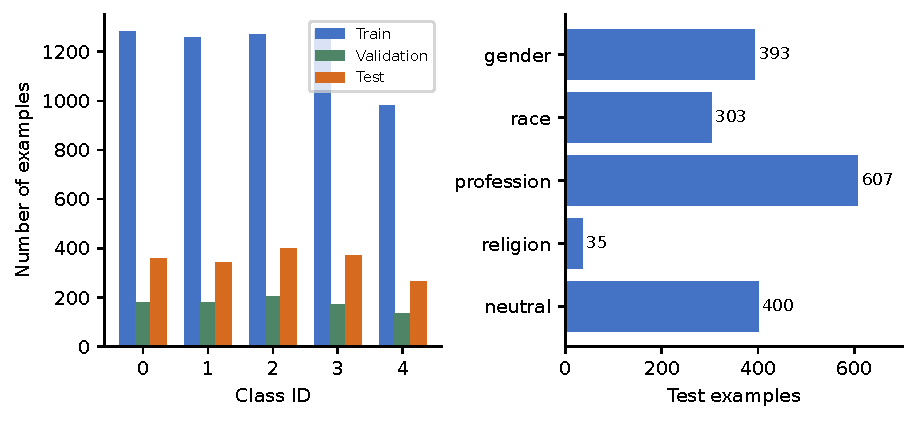
\includegraphics[width=\linewidth]{figures/dataset_distribution.pdf}
\caption{Class counts across splits (left) and normalized category counts in test (right). Class IDs follow Table~\ref{tab:dataset}.}
\label{fig:distribution}
\end{figure}

\subsection{Preprocessing and data-quality audit}
The model workflows preserve the supplied split assignments and numeric labels. Encoder tokenization uses padding, a 128-token limit, and model-specific special tokens. The saved encoder training records report no truncation of the original sentences. The Qwen training configurations use their own prompt-length limits; the annotation-conditioned and JSON SFT configurations record a 512-token maximum. Labels and other gold outputs are excluded from inference prompts according to the selected task.

A report-generation audit of sentence strings, after trimming only leading and trailing whitespace, finds no empty sentences. It finds 10 duplicate sentence rows in training, none in validation, and one in test. Five distinct training sentences and one distinct test sentence have more than one associated label. The audit also finds one distinct shared sentence between training and validation, four between training and test, and none between validation and test. One of the four train/test shared sentences has different label sets across those splits.

These observations describe the supplied files. The reported evaluations use their original split assignments and annotations.
